\documentclass[a4paper,11pt]{article}

\usepackage[utf8]{inputenc}

\usepackage{graphicx}
\usepackage{caption}
\usepackage{subcaption}

\usepackage{pgfplots}
\usepackage{float}
\usepackage{hyperref}
\usepackage{soul}
\hypersetup{
    colorlinks=true, % Enable colored links
    linkcolor=black, % Color for internal links
    urlcolor=black,  % Color for external links
    citecolor=black, % Color for citation links
    pdfborder={0 0 0}, % Remove border around links
}
\newcommand{\underlinehref}[2]{%
    \href{#1}{\ul{#2}}%
}
\pgfplotsset{compat=1.18}


\usepackage{minted}

\begin{document}

    \title{
        \textbf{Linked lists in C}
    }
    \author{Péter Herczku}
    \date{Fall 2024}

    \maketitle

    \section*{Introduction}

    The task is to implement the Linked List data structure and benchmark various operations on them as well as discussing the implementation of the stack data structure using a linked list under the hood.
    The complete code for the benchmarks can be found at the end of this report.

    I completed the assignment using the C programming language.

    \section*{Linked list}

    The idea behind linked data structures is that each element points to the next one in the list.
    This allows the elements to be stored anywhere in memory, not particularly after each other.

    A linked list holds a sequence of data items, but it only has access to the first element.
    Then, the first element has access to the second one, so on and so forth.
    Each element in the list is a data structure containing the value it holds, and a pointer to the next element in the sequence.
    The last element in the list points to a {\tt NULL} pointer.
    We must be careful regarding this {\tt NULL} pointer, because dereferencing it could lead to serious issues during runtime.

    Let's look at our implementation of linked list, completing the skeleton code provided in the description of the assignment:

    \begin{minted}{c}
void add(linked *lnk, int item) {
    cell *newCell = (cell*)malloc(sizeof(cell));
    newCell->value = item;
    newCell->tail = lnk->first;
    lnk->first = newCell;
}
    \end{minted}

    We allocate a new cell on the heap, link it to the head of the linked list, and attach the rest of the list.

    \begin{minted}{c}
int length(linked *lnk) {
    int i = 0;
    cell* current = lnk->first;
    while(current != NULL) {
        i++;
        current = current->tail;
    }
    return i;
}
    \end{minted}

    We traverse the linked list until we reach the null pointer.

    \begin{minted}{c}
bool find(linked *lnk, int item) {
    cell* current = lnk->first;
    while(current != NULL) {
        if(current->value == item) return true;
        current = current->tail;
    }
    return false;
}
    \end{minted}

    This method is similar to the {\tt length} function, but we are checking the current value of the cell, and return if it's the same as the item we are looking for.

    \begin{minted}{c}
void removeItem(linked *lnk, int item) {
    cell* prev = NULL;
    cell* current = lnk->first;
    while(current != NULL) {
        if(current->value == item) {
            if(prev == NULL) {
                lnk->first = current->tail;
            } else {
                prev->tail = current->tail;
            }
            free(current);
            return;
        }
        prev = current;
        current = current->tail;
    }
}
    \end{minted}

    This function traverses the list to find and remove an element with the value {\tt item}.
    If the element is found, it gets removed by attaching the previous and the next element to each other.

    \section*{Appending lists}

    In the assignment we are asked to create a function that appends a linked list B to another linked list A.
    Let's look at our implementation of this function:

    \begin{minted}{c}
void append(linked *a, linked *b) {
    cell *nxt = a->first;
    cell *prv = NULL;
    while(nxt != NULL) {
        prv = nxt;
        nxt = nxt->tail;
    }
    if (prv != NULL) {
        prv->tail = b->first;
    } else {
        a->first = b->first;
    }
    b->first = NULL;
}
    \end{minted}

    We essentially traverse the linked list A, looking for the last element.
    Then, we attach the head of B to the end of A, and disconnect the head from linked list B.

    \subsection*{Keeping the size of B constant}

    Let's do some benchmarks to see how runtime varies for different sizes.
    In the first case, we will be varying the size of A, keeping the size of B constant.
    We need to traverse through A to reach the end of the list.
    During this we are doing $O(1)$ operations n times, therefore our expected time complexity is $O(n)$.

    \begin{figure}[h]
        \centering
        \begin{subfigure}[b]{.5\textwidth}
            \centering
            \includegraphics[width=\textwidth]{./benchmark/data} % Adjust width or height as needed
        \end{subfigure}
        \caption{Graph of keeping the size of B constant}
        \label{fig:graph_1}
    \end{figure}

    As we can see, the graph clearly shows linear relationship, therefore our theoretical assumption of time complexity was correct, and is indeed $O(n)$.

    \subsection*{Keeping the size of A constant}

    If we keep the size of A constant, the time complexity should be $O(1)$, since we don't need to traverse B to attach it to A.
    Let's run some benchmarks to validate our point:

    \begin{figure}[h]
        \centering
        \begin{subfigure}[b]{.5\textwidth}
            \centering
            \includegraphics[width=\textwidth]{./reverse_append/data} % Adjust width or height as needed
        \end{subfigure}
        \caption{Graph of keeping the size of A constant}
        \label{fig:graph_2}
    \end{figure}

    We can observe constant runtime from the graph when we are varying the size of B\@.

    \subsection*{Comparing it to arrays}

    If we want to append array B to array A, we need to iterate through B and push them one by one to the array A.
    During this we might need to allocate more memory for the array A as well.
    However, since we are dealing with arrays, reading elements from B is very fast.
    When the first element is being read, the CPU loads the other elements into its cache as well.
    Writing to array A is also very efficient, as we do not need to wait for the write operation to complete, we can just move on to the next element.

    \section*{Stack using a linked list}

    In order to get good performance, the head of the linked list would be the top of the stack, because when we are adding an element to the beginning of the linked list, it is done in $O(1)$ time complexity, therefore we can use our already written {\tt add} function for the {\tt push} operation.
    The implementation of the {\tt pop} operation is also very straightforward, we just need to attach the tail of the first element to the head of the linked list.
    However, we need to allocate memory on each push operation, and free memory on each pop operation, which could increase our runtime.

    Using arrays, both popping and pushing elements onto the stack is also done in $O(1)$ time complexity, but without memory overhead.
    Hence, our runtime should be slightly better using arrays instead of linked lists.

    \section*{GitHub}
    I have uploaded the full project to \underlinehref{https://github.com/peterherczku/ID1021/tree/main/assignment-5}{my github repository}, where we can find the code used to make this report.

\end{document}
